%\newpage
%\thispagestyle{empty}
%\mbox{}

\chapter{Resultados experimentales}
\label{ch:chapter3}

Una vez sentadas las bases del sistema en su totalidad, se estudiarán diversos comportamientos que irán apareciendo en función de variar cada uno de sus parámetros. Entre ellos estarían evaluar el avance de la formación empezando en diversos puntos del espacio, variar el número de agentes $N$, modificar el radio de la formación $D$, probar diferentes valores de la ganancia $\epsilon$ y finalmente probar su fiabilidad en superficies con múltiples fuentes.

Para ello, la simulación va a basarse en la  siguiente función gaussiana:

\begin{equation}\label{Funcion_Gaussiana_2} 
	f\left(x,y\right) = p\cdot{e}^{-\left(c-c_o\right)^{T}\cdot{M}\cdot\left(c-c_{o}\right)},
\end{equation}

en donde, $c=\left(x,y\right)$ es el valor en el centro de la formación, $c_o=\left(x_{o},y_{o}\right)$ sería la posición del centro de la gaussiana. Cabe destacar que se dio una descripción más detallada en la sección \ref{Simulacion_Modelo}.

Para los primeros 4 casos se particulariza la simulación del sistema en base a los siguientes datos: el centro se situé en $c_{o}=[600,600]$, el ángulo $\theta$ nulo, una desviación uniforme en ambos ejes $\sigma_{x}=\sigma_{y}=\frac{1}{1000}$ para que la matriz quede definida como $S = \bigl[\begin{smallmatrix}\frac{1000}{\sqrt{2}} & 0\\ 0 & \frac{1000}{\sqrt{2}}\end{smallmatrix}\bigr]$  y cuyo volumen es $p = 1$.

Se van a emplear 4 vehículos que parten de posiciones arbitrarias y convergen situado en el origen. El gradiente estimado, es en realidad las sucesivas posiciones de los centros de la formación circular descrita por los vehículos cuyo radio $D$ será 30, y desplazados siguiendo el algoritmo de ascenso de gradiente con una ganancia $\epsilon$=20.

En primer lugar, se demostrará el correcto funcionamiento de la coordinación ejercida por los vehículos a través de la siguiente figura:

\begin{figure}[H]
  \begin{center}
    \subfigure[Situación inicial]{
        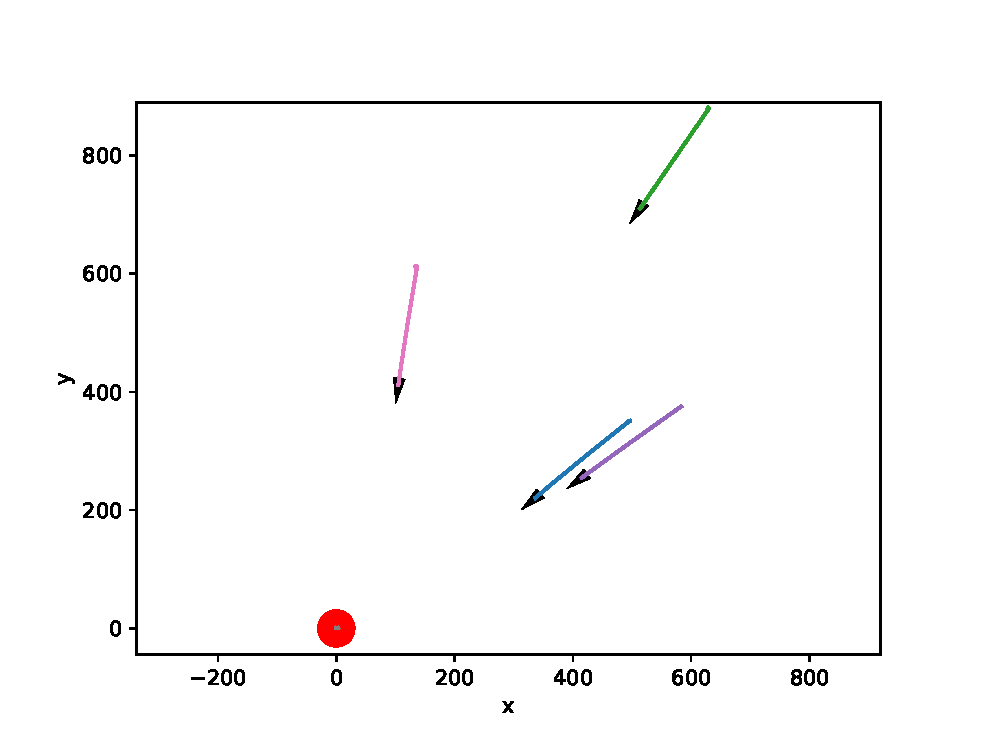
\includegraphics[width=0.43\textwidth]{figures/Cap_3/Pos_Aleatorias.eps}
        \label{Inicio_Posiciones}}
    \subfigure[Avance]{
        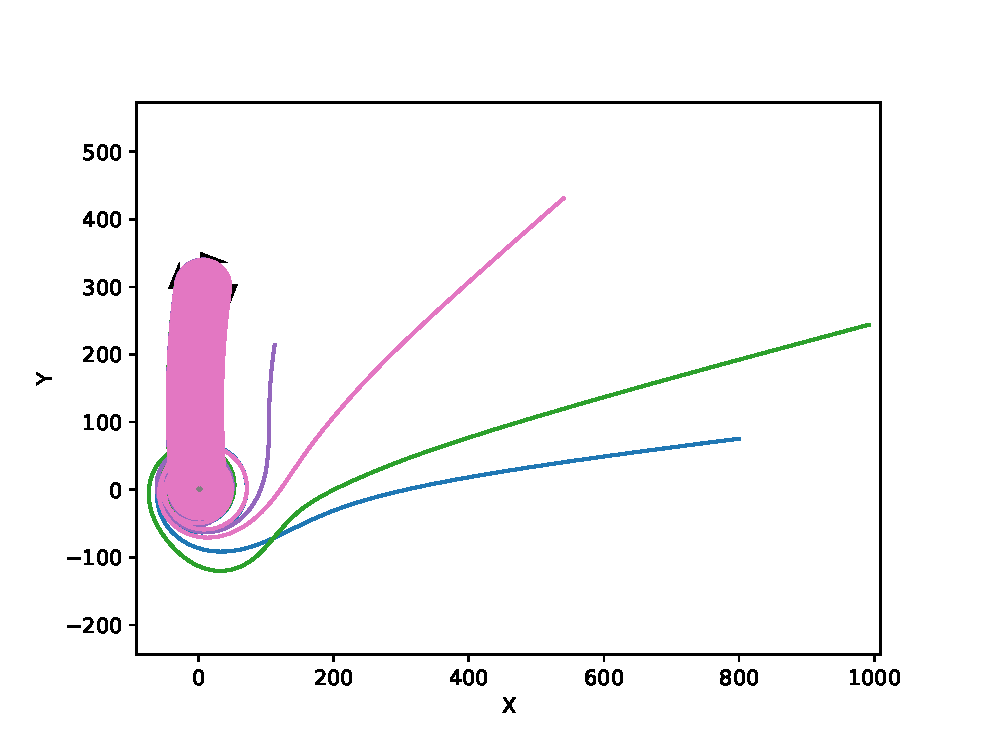
\includegraphics[width=0.43\textwidth]{figures/Cap_3/Avance.eps}
        \label{Avance_Circulitos}}
    \caption{Vehículos dispuestos en torno a la formación. El punto rojo representa el círculo al que quieren converger y las diferentes líneas de colores que giran en torno a dicho punto son cada una de las trayectorias de los vehículos.}
    \label{Demostracion_Coordinacion}
  \end{center}
\end{figure}
Un comentario destacable es que se deben imponer dos condiciones que necesariamente se deben cumplir para que el sistema avance satisfactoriamente. Estas son:

\begin{itemize}
	\item La primera es que el error de formación sea lo más próximo a 0 posible, es decir, que en la medida de lo que cabe los vehículos estarán dispuestos uniformemente en la circunferencia pero con un error que se adicionará al existente por la estima del gradiente. Por ello, se decide imponer que como mucho $e_{\theta}\leq{0.2}$ sobre la ecuación \ref{Error_Coordinacion}.
	\item La segunda consiste en dar una solución satisfactoria para tomar en consideración que ya se ha llegado al punto de interés. Esto se debe a la dificultad de movimiento cuando estés muy cerca del máximo al gradiente hacerse prácticamente 0 y, por lo tanto la formación apenas avanza. Por ello, se impone que para satisfacer condición de máximo será solución al problema cuando $f(c)\geq{0.999}$.
\end{itemize}

Puede darse el caso de que la ultima de las condiciones no se cumpla. Esto se debe a que el máximo se encontraría definido en una zona plana, y por ende el avance por dicha zona se volvería inviable. Para solucionarlo, basta con imponer que se ha llegado satisfactoriamente al máximo si se lee continuamente el mismo valor sobre la función \ref{Funcion_Gaussiana_2} y a su vez el valor del gradiente es próximo a cero. 

A continuación, se reflejará el camino siguiendo al gradiente estimado en comparación con el camino siguiendo el gradiente real, la evolución de cada componente del gradiente hasta llegar al punto máximo y finalmente una curva de error que posteriormente se definirá.

\begin{figure}[H]
\centering
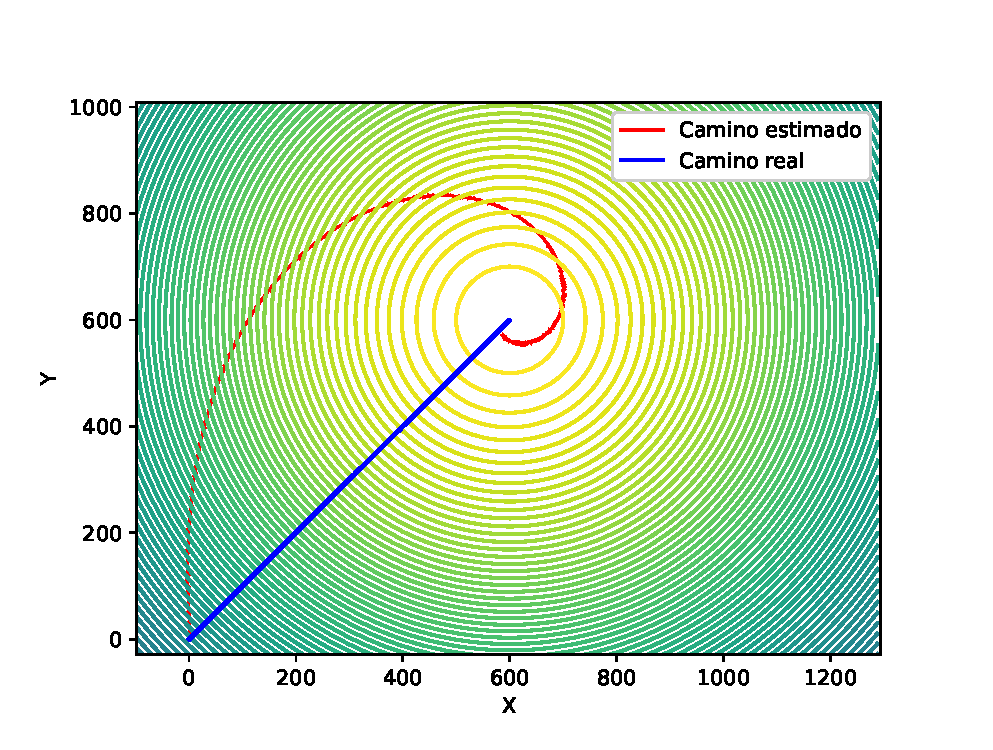
\includegraphics[width=0.70\textwidth]{figures/Caso_Inicial/Caminos.eps}
\caption{Comparativa entre el camino descrito por el gradiente real y por el gradiente estimado.} \label{Dif_Caminos}
\end{figure}

\begin{figure}[H]
\centering
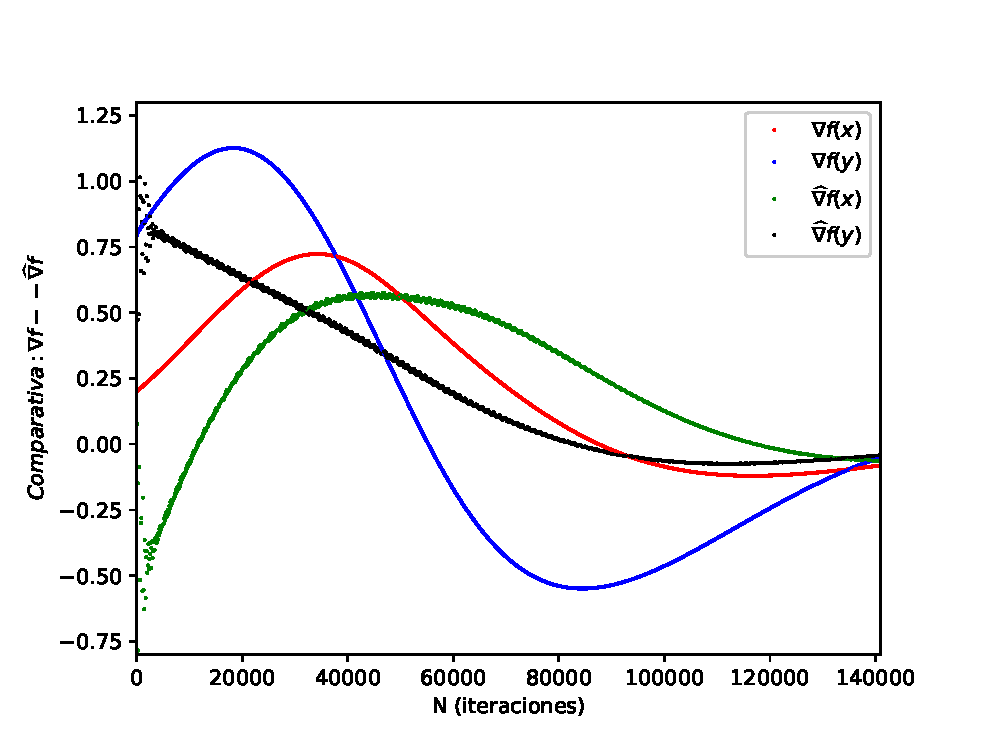
\includegraphics[width=0.58\textwidth]{figures/Graficas_Nuevas/Caso_Inicial/Figure_3.eps}
\caption{Comparativa de las componentes del gradiente entre el real y el estimado.} \label{grad}
\end{figure}

\begin{figure}[H]
\centering
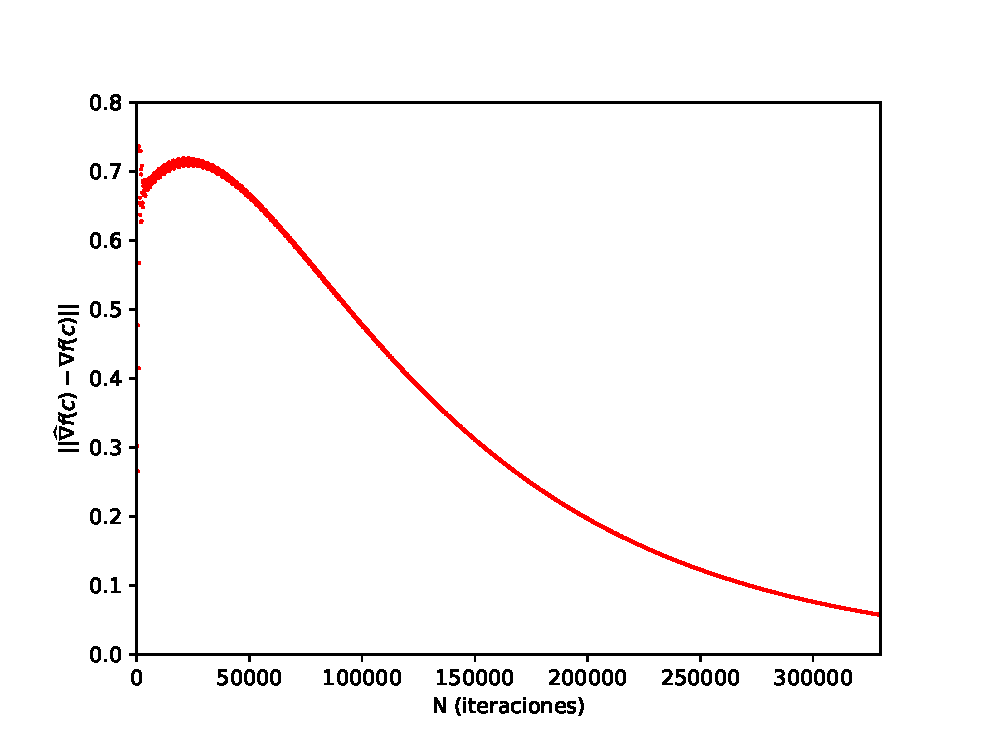
\includegraphics[width=0.58\textwidth]{figures/Graficas_Nuevas/Caso_Inicial/Figure_5.eps}
\caption{Curva de error descrita por la estimación del gradiente.} \label{Curva_error}
\end{figure}

En la figura \ref{Dif_Caminos} se aprecia como claramente el avance obtenido por el gradiente estimado difiere del real pasando de una recta a definir prácticamente una espiral. Esto era un resultado bastante esperable al acumular un error equiparable al orden 2 de Taylor visto en la ecuación \ref{Fun_Esti}, además se adiciona el error del angulo entre vehículos visto en \ref{Error_Coordinacion} que provocará una estima del gradiente incluso más alejada de lo ideal. 

Por otro lado, en la figura \ref{grad} se observa la variación de cada componente del  gradiente real frente al estimado, a pesar de que difieren notablemente se aprecia como al avanzar el sistema ambos gradientes convergen al mismo punto. Esto se traduce en que el gradiente estimado es capaz de guiar a la formación al punto con máxima concentración de sustancias.

Acudiendo a la referencia \cite{Estimacion_Gradiente} se aproxima al error existente entre ambos gradientes como:

\begin{equation} \label{error_gradiente}
	\Delta{\nabla{f\left(c\right)}}=||\hat{\nabla}f\left(c\right)-\nabla{f}\left(c\right)||
\end{equation}

La figura \ref{Curva_error} describe el error dado por la ecuación \ref{error_gradiente}. Se nota como según más próximo a la fuente este la formación su valor tiende asintóticamente a 0. Esta ecuación se va a utilizar para evaluar el rendimiento del sistema frente a variar sus parámetros, tal como se ha comentado en diversas ocasiones a lo largo de la memoria.

\section{Variación del punto inicial}
\begin{figure}[H]
\centering
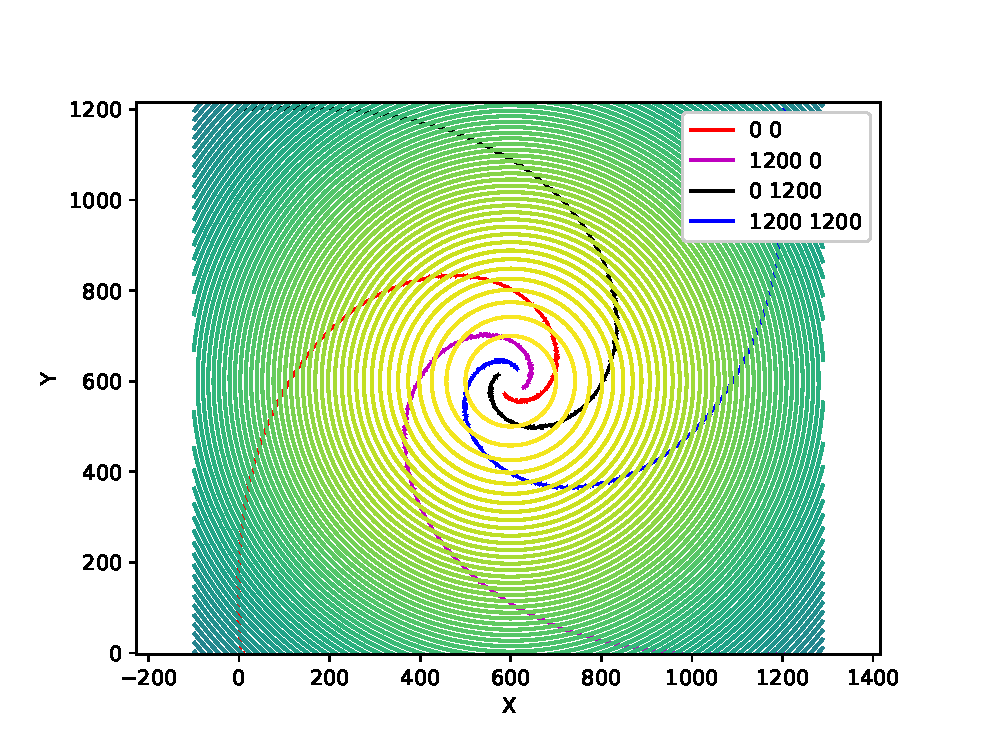
\includegraphics[width=0.62\textwidth]{figures/4_puntos_observar_forma/Figure_1.eps}
\caption{Avance del sistema para diferentes valores de la posición inicial de la formación.} \label{Avance_Posicion}
\end{figure}

La primera situación planteada consiste en utilizar los datos descritos anteriormente\footnote[2]{N = 4, D = 30 y $\epsilon$=20} para evaluar el efecto que tiene partir desde diferentes puntos. Consecuentemente, se escogen cuatro vértices que forman una diagonal respecto al punto máximo siendo estos $x_o=[0,1200]$, $x_o=[1200,0]$, $x_o=[1200,1200]$ y el origen. El resultado esperable es que la trayectoria descrita posea el mismo punto final\footnote[3]{Máxima concentración de sustancias}, pero lo hará definiendo otra forma, tal como se observo en \ref{Dif_Caminos}. Finalmente, se contempla en la figura \ref{Gradiente_Diversos_Puntos} que las iteraciones persisten para cada punto de partida, por ende el error terminaría siendo similar a \ref{Curva_error} en todos los casos. 

\begin{figure}[H]
  \begin{center}
    \subfigure[Punto 0 0]{
        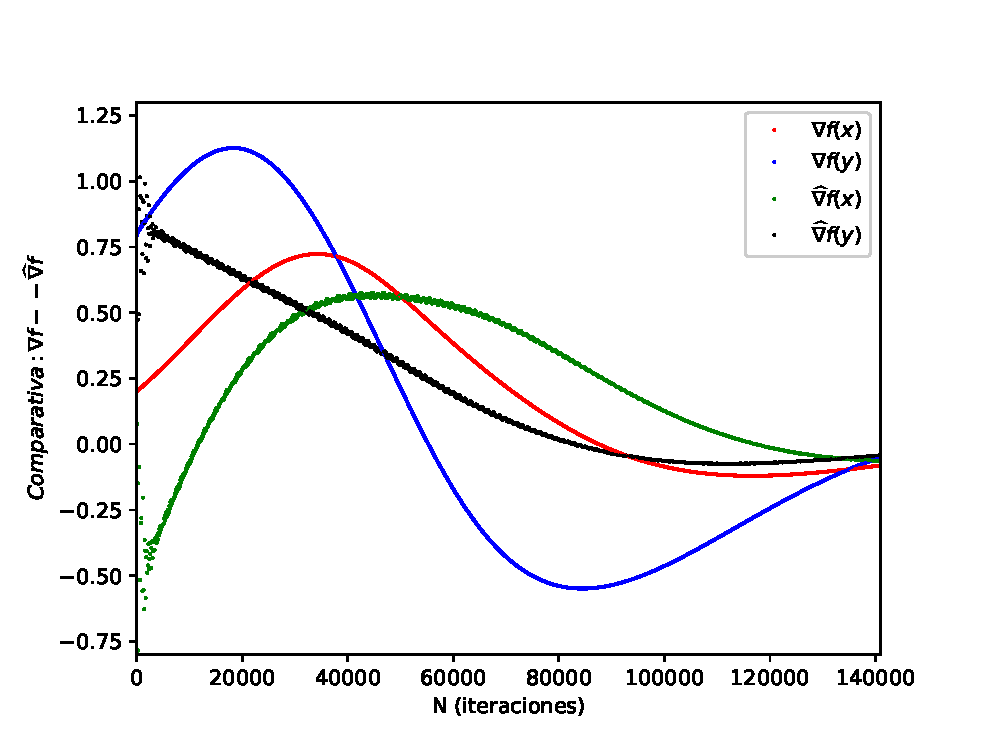
\includegraphics[width=0.45\textwidth]{figures/Graficas_Nuevas/Caso_Inicial/Figure_3.eps}
        }
    \subfigure[Punto 0 1200]{
        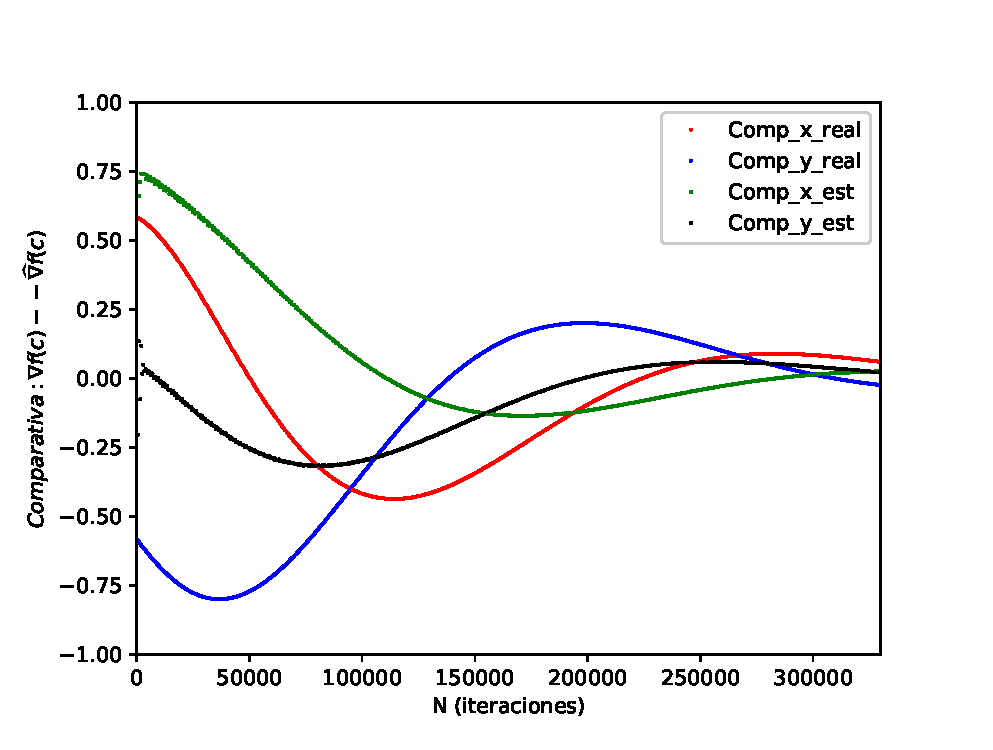
\includegraphics[width=0.45\textwidth]{figures/Graficas_Nuevas/Posicion/0_1200.eps}
        }
	\subfigure[Punto 1200 0]{
        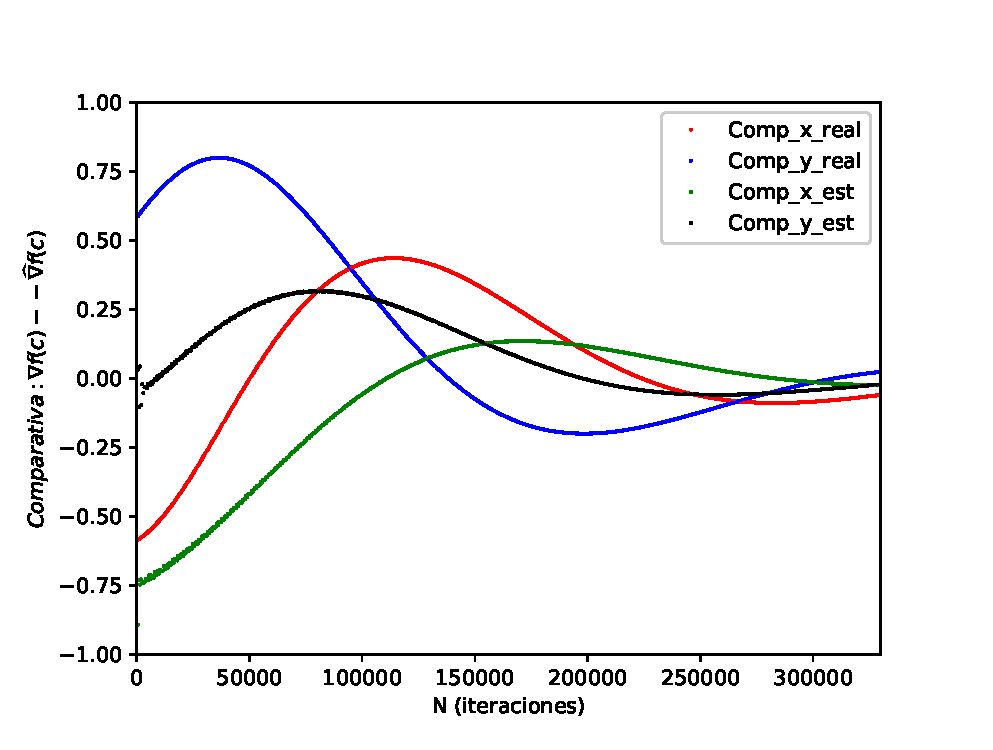
\includegraphics[width=0.45\textwidth]{figures/Graficas_Nuevas/Posicion/1200_0.eps}
        }
	\subfigure[Punto 1200 1200]{
        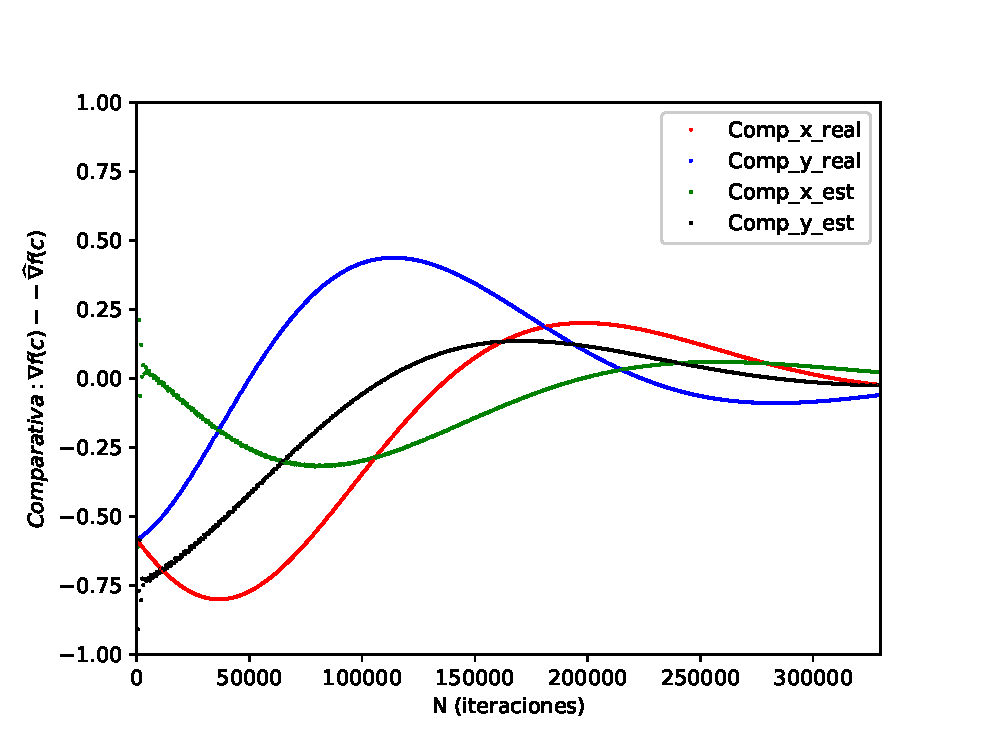
\includegraphics[width=0.45\textwidth]{figures/Graficas_Nuevas/Posicion/1200_1200.eps}
        }
    \caption{Componentes del gradiente estimado y el real para diferentes valores de la posición inicial de la formación.}
    \label{Gradiente_Diversos_Puntos}
  \end{center}
\end{figure}

\section{Variación del número de agentes N}

\begin{figure}[H]
\centering
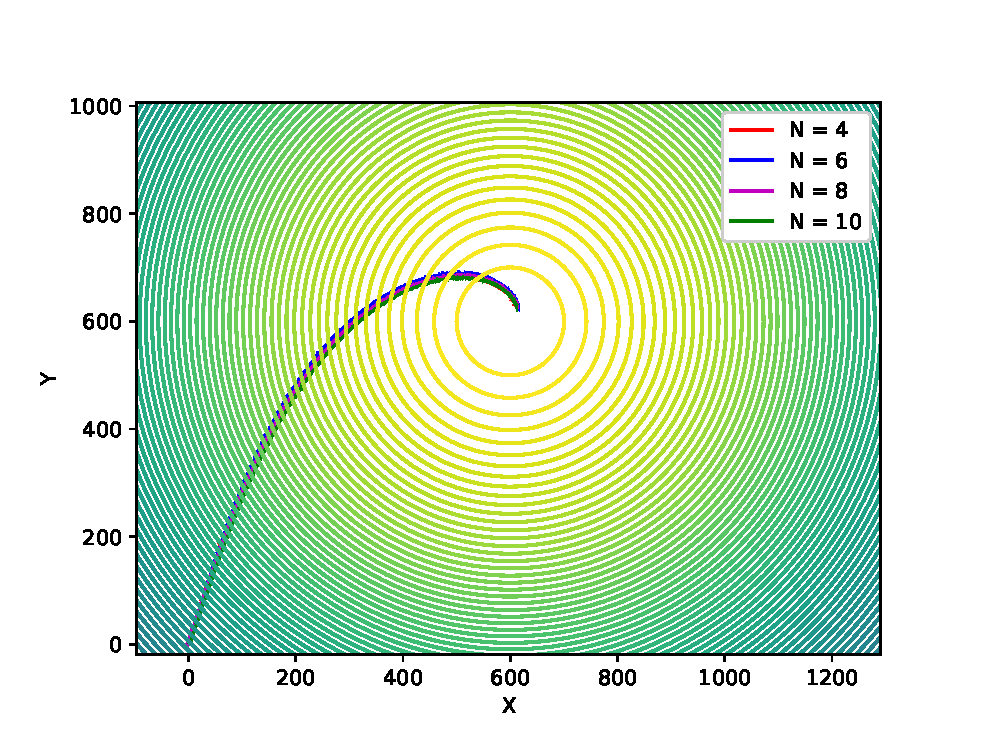
\includegraphics[width=0.65\textwidth]{figures/N_Var_R_50/Figure_1.eps}
\caption{Avance del sistema en función del número de agentes N.} \label{N_Var}
\end{figure}

El número de agentes va a influir de dos maneras: 

\begin{enumerate}
	\item Este primer resultado se podía intuir de la gráfica \ref{NAGENTSEST}, en donde claramente se aprecia una dependencia inversamente proporcional, es decir, a medida que se aumenta el número de agentes es de esperarse que el error se reduzca y a su vez las iteraciones necesarias para llegar al máximos se reducen.
	\item No obstante, si se tiene en cuenta el algoritmo de control de formación  cada vez que el número de agentes va creciendo se tienen más nodos dentro del sistema y por ello se ha de pasar mucha más información al presentar más nodos adyacentes, traduciéndose en una ralentización en la coordinación de los vehículos. A esto se le añade el tiempo que se tendría que esperar para que los $N$ vehículos se dispongan uniformemente en la formación.
\end{enumerate}

Se puede apreciar como la trayectoria descrita en \ref{N_Var} no cambia significativamente. Sin embargo, si tiene un impacto en el número de iteraciones \ref{Gradiente_N_Var} y en la reducción del error \ref{N_Var_Error}. Para este último caso, se tiene que a partir de un determinado número de agentes la influencia sobre el sistema se hace prácticamente inapreciable.

\begin{figure}[H]
  \begin{center}
    \subfigure[N = 4]{
        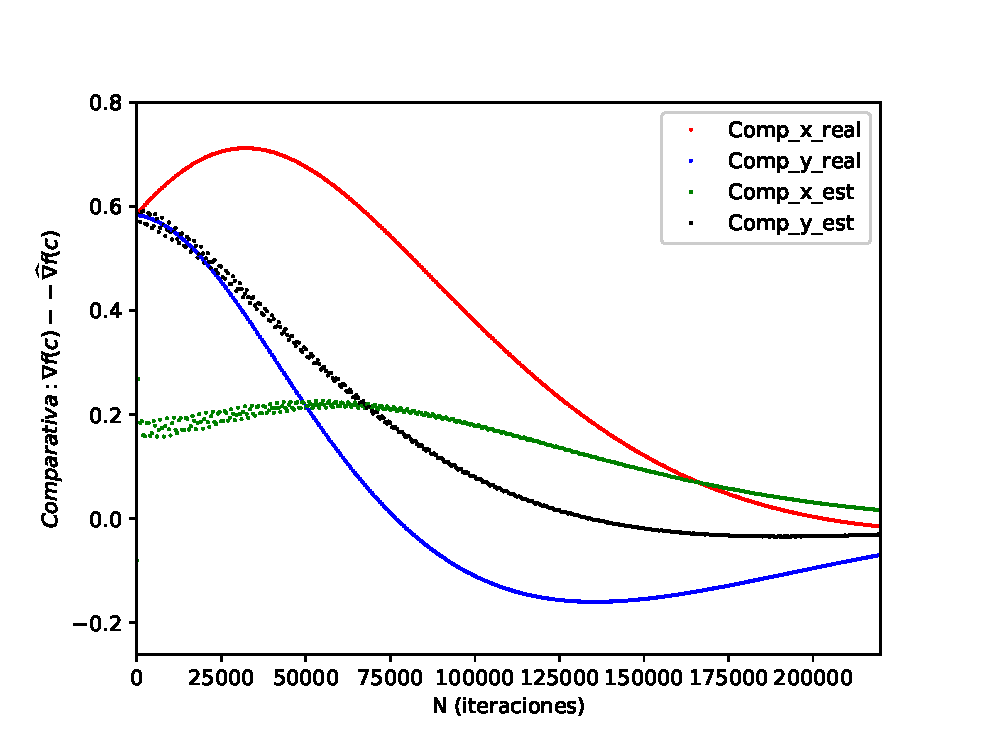
\includegraphics[width=0.45\textwidth]{figures/Graficas_Nuevas/N/N4.eps}
        }\label{N4}
    \subfigure[N = 6]{
        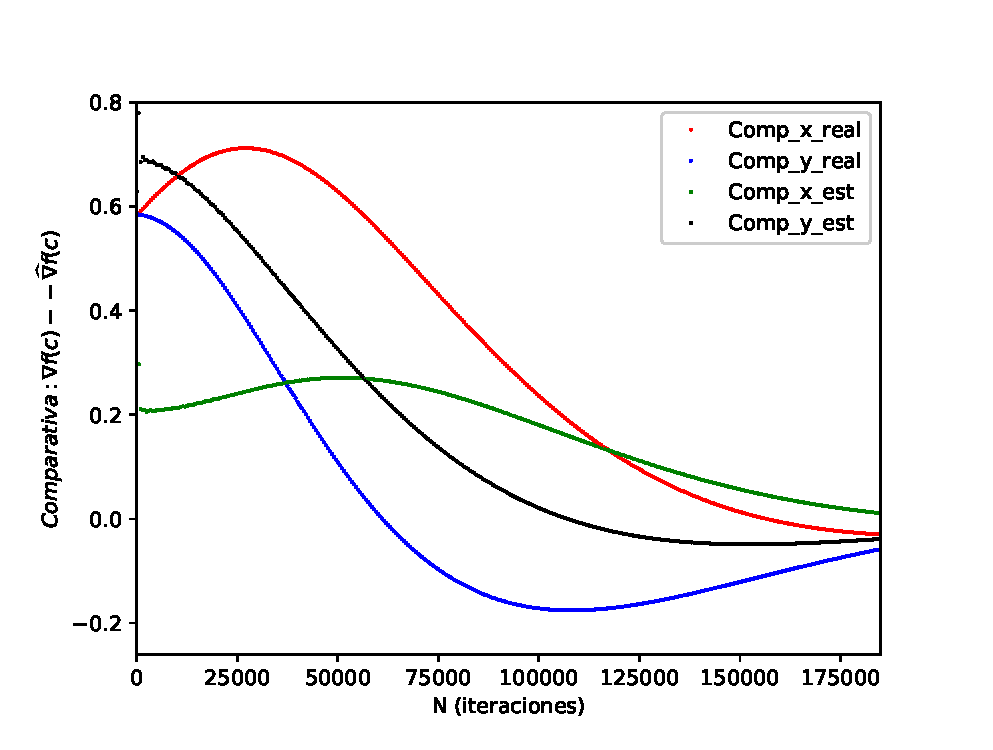
\includegraphics[width=0.45\textwidth]{figures/Graficas_Nuevas/N/N6.eps}
        }
	\subfigure[N = 8]{
        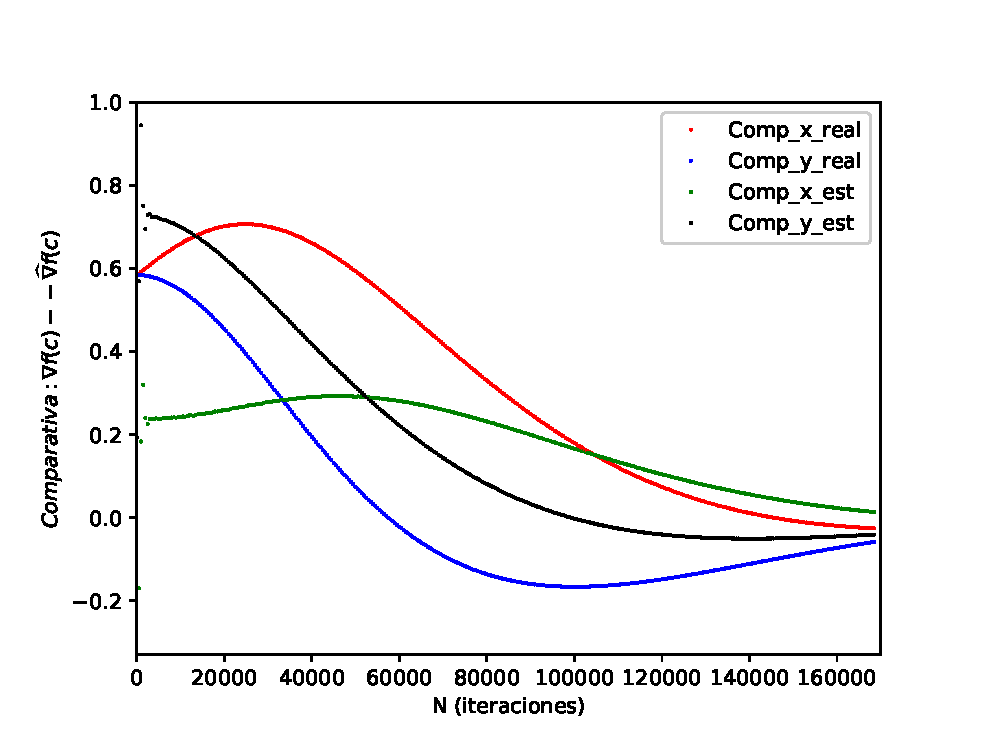
\includegraphics[width=0.45\textwidth]{figures/Graficas_Nuevas/N/N8.eps}
        }
	\subfigure[N = 10]{
        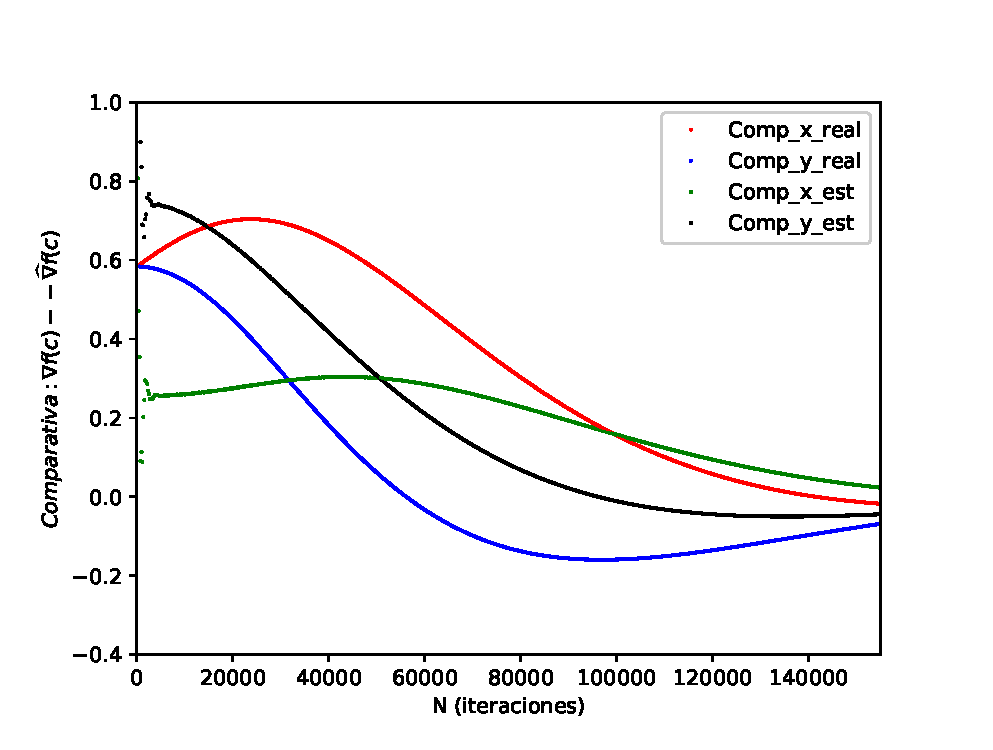
\includegraphics[width=0.45\textwidth]{figures/Graficas_Nuevas/N/N10.eps}
        }
    \caption{Evaluación de las componentes del gradiente estimado y el real en función del número de agentes N.}
    \label{Gradiente_N_Var}
  \end{center}
\end{figure}

Adicionalmente, se aprecia en la figura \ref{N4} que al principio las componentes del gradiente estimado presentan oscilaciones en sus valores. Dicho efecto se mitiga según se aumenta el número de agentes.

\begin{figure}[H]
\centering
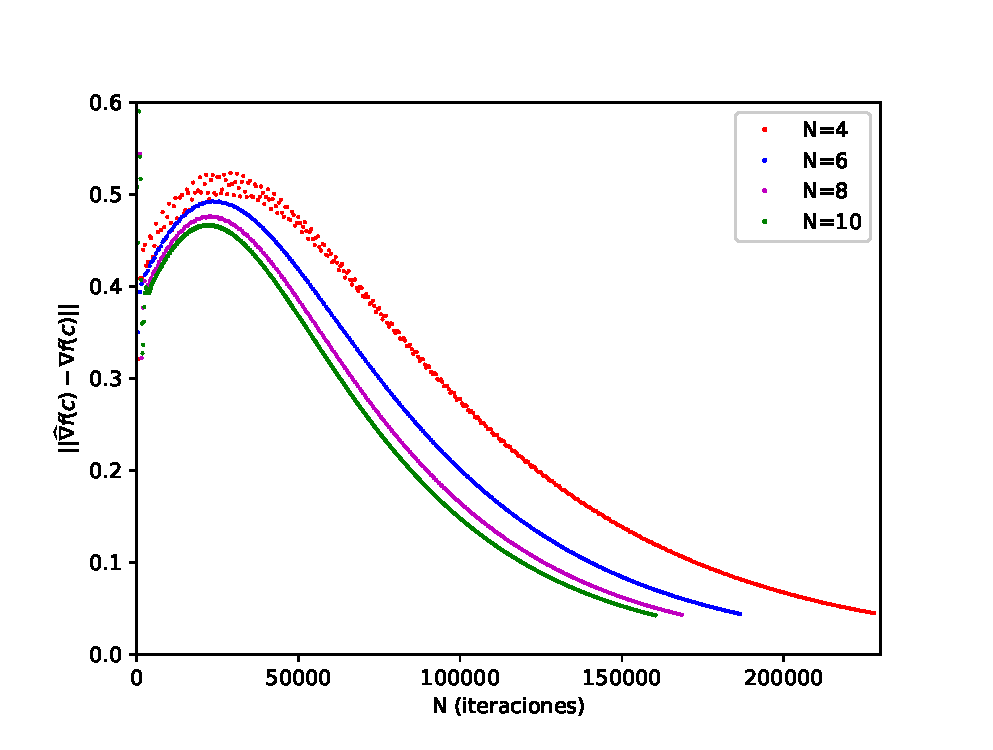
\includegraphics[width=0.66\textwidth]{figures/Graficas_Nuevas/N/Figure_5.eps}
\caption{Error descrito por el gradiente estimado al variar el número de agentes N.} \label{N_Var_Error}
\end{figure}

\section{Variación del radio D}

\begin{figure}[H]
\centering
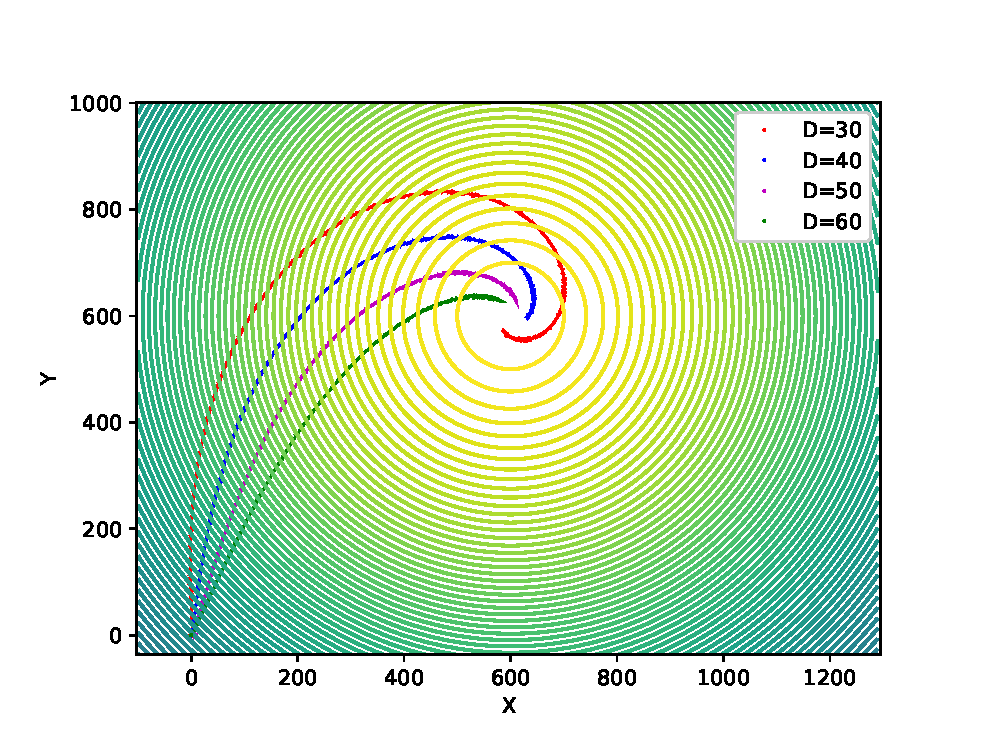
\includegraphics[width=0.66\textwidth]{figures/Dif_R_BU/Figure_1.eps}
\caption{Avance del sistema en función del radio D.} \label{D_Var}
\end{figure}

Imponiendo que N = 4 y $\epsilon$=20, se evalúa la influencia del radio D. Se aprecia que el sistema en sí es mucho más sensible al radio de la formación que al número de agentes. En la referencia \cite{Adicional_Estimacion_1} acota al error de la siguiente forma:
\begin{equation}\label{Depe}
	||\hat{\nabla}f\left(c\right)-\nabla{f}\left(c\right)||\leqslant{D·L},
\end{equation}

en donde, $L$ es un escalar delimitado por el error de la serie de Taylor original. Si bien es cierto que el error depende del radio de la formación D de tal forma que un aumento conlleva a tener más error al darle mayor margen sobre la desigualdad \ref{Depe}.

\begin{figure}[H]
  \begin{center}
    \subfigure[D = 30]{
        \includegraphics[width=0.45\textwidth]{figures/Graficas_Nuevas/D/D30.eps}
        }
    \subfigure[D = 40]{
        \includegraphics[width=0.45\textwidth]{figures/Graficas_Nuevas/D/D40.eps}
        }
	\subfigure[D = 50]{
        \includegraphics[width=0.45\textwidth]{figures/Graficas_Nuevas/D/D50.eps}
        }
	\subfigure[D = 60]{
        \includegraphics[width=0.45\textwidth]{figures/Graficas_Nuevas/D/D60.eps}
        }
    \caption{Evaluación de la componentes del gradiente estimado y el real en función del radio D.}
    \label{Gradiente_Var_D}
  \end{center}
\end{figure}

En la formación de control va a influir directamente el radio de la circunferencia dado que entre mayor sea D el error prefijado será menos restrictivo y por ende aprecias comportamientos oscilantes en las zonas lejanas al máximo de radiación.

Evaluando únicamente al radio D se ve como a medida que su valor decrece el error aumenta y con ello el número de iteraciones de una forma mucho más notoria que el número de agentes. 

\begin{figure}[H]
\centering
\includegraphics[width=0.70\textwidth]{figures/Graficas_Nuevas/D/DVariable.eps}
\caption{Error descrito por el gradiente estimado al variar el radio D.} \label{D_Var_Error}
\end{figure}

\section{Variación de la constante $\epsilon$}

Este caso va a estar estrictamente relacionado con \ref{GA} dado que si se aumenta el valor de $\epsilon$ es de esperarse que la formación avance más en la dirección del gradiente, de modo que la formación llegue más rápido al punto máximo. No obstante, al aumentar la ganancia que multiplica al gradiente a su vez estás arrastrando al error provocando que la trayectoria descrita por la espiral se acentué mucho más. Este efecto es apreciable en la figura \ref{Epsilon_Var}.

\begin{figure}[H]
\centering
\includegraphics[width=0.72\textwidth]{figures/Epsilon_variante/Figure_1.eps}
\caption{Avance del sistema en función del radio peso $\epsilon$.} \label{Epsilon_Var}
\end{figure}

\begin{figure}[H]
\centering
\includegraphics[width=0.72\textwidth]{figures/Graficas_Nuevas/E/EPSILONVAR2.eps}
\caption{Error descrito por el gradiente estimado al variar el peso $\epsilon$.} \label{Epsilon_Var_Error}
\end{figure}

El comportamiento de la ganancia $\epsilon$ presenta un efecto diferente sobre el gradiente estimado y sobre el gradiente real, en el primero de estos es apreciable  en la figura \ref{Epsilon_Var_Error} que aumentarlo es perjudicial para el algoritmo dado que conllevaría a elevar en exceso tanto el número de iteraciones como $\Delta{\nabla{f\left(c\right)}}$. Este efecto era justo el contrario con el gradiente real, en donde si aumentas el valor de dicha ganancia se daban casos donde llegabas con menos pasos al máximo.

\begin{figure}[H]
  \begin{center}
    \subfigure[$\epsilon$ = 20]{
        \includegraphics[width=0.41\textwidth]{figures/Graficas_Nuevas/E/E20.eps}
        }
    \subfigure[$\epsilon$ = 50]{
        \includegraphics[width=0.41\textwidth]{figures/Graficas_Nuevas/E/E50.eps}
        }
	\subfigure[$\epsilon$ = 80]{
        \includegraphics[width=0.41\textwidth]{figures/Graficas_Nuevas/E/E80.eps}
        }
    \caption{Evaluación de las componentes del gradiente estimado y el real en función del peso $\epsilon$.}
    \label{Gradiente_Var_Epsilon}
  \end{center}
\end{figure}

Finalmente, se procederá a evaluar un caso particular en el que se tienen múltiples fuentes emitiendo con el objetivo de demostrar las limitaciones que presenta la utilización del algoritmo de ascenso de gradiente.

\section{Evaluación con múltiples fuentes}

En este caso se va a considerar que N = 4, D = 50 y $\epsilon$=20, además el nuevo plano sobre el que se desplaza el enjambre se describe según:

\begin{itemize}
	\item Una primera gaussiana con los siguientes datos: el centro se situé en $c_{o}=[0,1200]$, un ángulo $\theta=0$ , una desviación uniforme en ambos ejes $\sigma_{x}=\sigma_{y}=\frac{1}{300}$ para que la matriz quede definida como $S = \bigl[\begin{smallmatrix}\frac{300}{\sqrt{2}} & 0\\ 0 & \frac{300}{\sqrt{2}}\end{smallmatrix}\bigr]$  y cuyo volumen es $p = 0.9$. 
	\item Una segunda gaussiana con los siguientes datos: el centro se situé en $c_{o}=[1200,0]$, un ángulo $\theta=0$ , una desviación uniforme en ambos ejes $\sigma_{x}=\sigma_{y}=\frac{1}{300}$ para que la matriz quede definida como $S = \bigl[\begin{smallmatrix}\frac{300}{\sqrt{2}} & 0\\ 0 & \frac{300}{\sqrt{2}}\end{smallmatrix}\bigr]$  y cuyo volumen es $p = 0.9$.
	\item Una tercera gaussiana con los siguientes datos: el centro se situé en $c_{o}=[600,600]$, un ángulo $\theta=\frac{\pi}{6}$ , una desviación distinta en cada eje con $\sigma_{x}=\frac{1}{1000}$ y $\sigma_{y}=\frac{1}{500}$  para que la matriz quede definida como $S = \bigl[\begin{smallmatrix}\frac{1000}{\sqrt{2}} & 0\\ 0 & \frac{500}{\sqrt{2}}\end{smallmatrix}\bigr]$ y cuyo volumen es $p = 1$. 
\end{itemize}

Todos estos datos referidos a lo visto en la sección \ref{Simulacion_Modelo}. Al sumarlas se obtiene:

\begin{figure}[H]
  \begin{center}
    \subfigure[Vista en 3D]{
        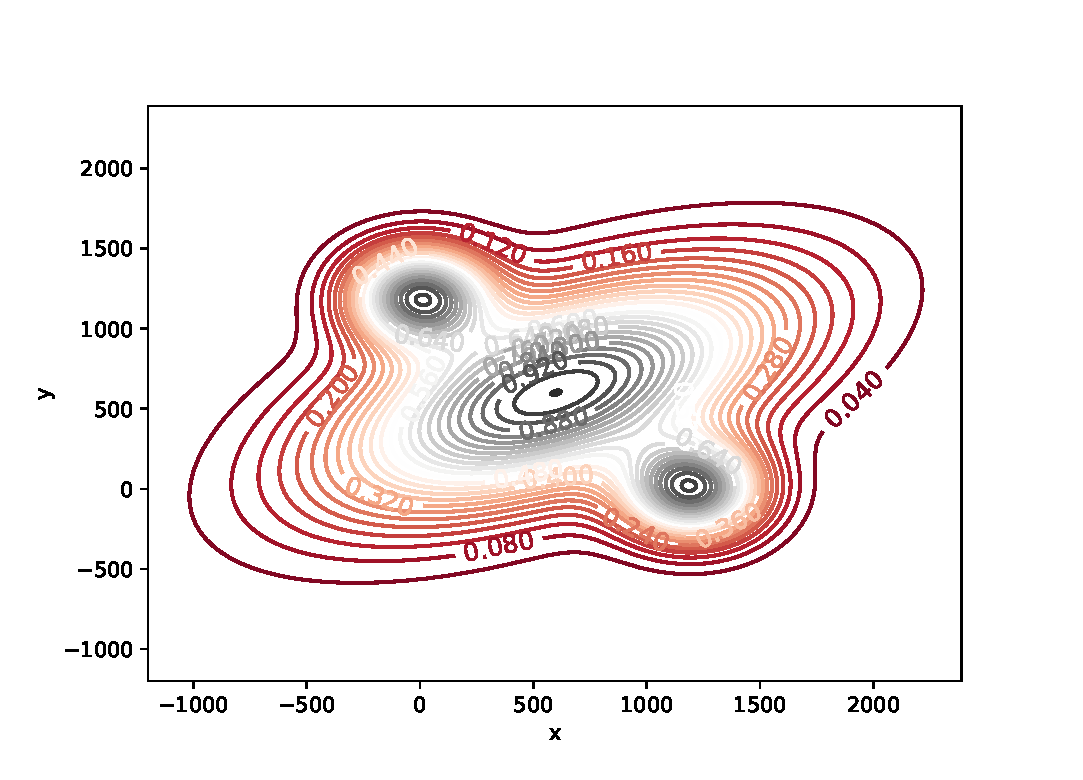
\includegraphics[width=0.45\textwidth]{figures/Casos_Especiales/Gaussiana.eps}
        }
    \subfigure[Curvas de nivel]{
        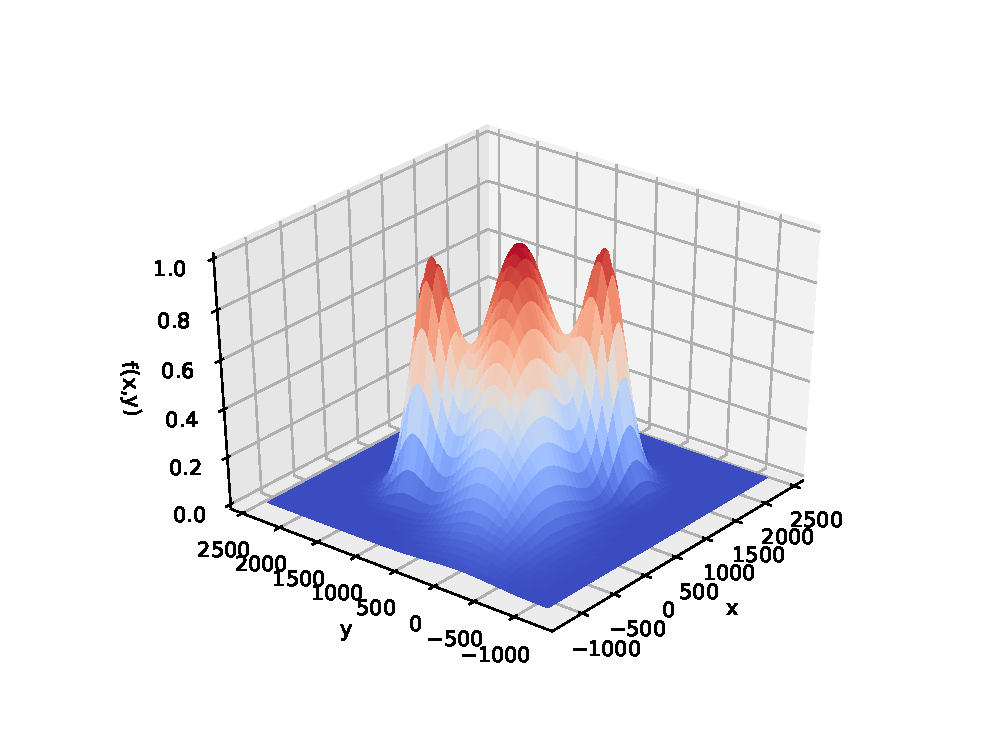
\includegraphics[width=0.45\textwidth]{figures/Casos_Especiales/Gaussiana_meh.eps}
        }
    \caption{Resultado de sumar las tres funciones gaussianas. Nuevo modelo para la simulación.}
    \label{New_Gaussiana}
  \end{center}
\end{figure}
\newpage
Con esta nueva función surgen dos casos de interés:

\begin{enumerate}
	\item El primero es que se tienen múltiples máximos, en concreto, dos locales y el global. Por lo que puede suceder que dependiendo del número de agentes N, el radio D o la ganancia $\epsilon$ vaya hacia cualquiera de los tres. Sin embargo, como ya se hizo un estudio de la influencia de cada parametro, directamente se evalúan las posiciones de partida del enjambre para observar hacia que fuente de emisión converge.
	\item El segundo son los dos puntos silla generados entre los tres máximos. Estos haciendo uso del gradiente real conformaban un problema al utilizar el algoritmo de ascenso de gradiente al hacerse $\nabla{f\left(c\right)}=0$. No obstante, se verá que en este caso eso no va a suceder.
\end{enumerate}
	
\begin{figure}[H]
\centering
\includegraphics[width=0.75\textwidth]{figures/Multi_Gaussiana/Figure_1.eps}
\caption{Avance definido sobre el plano con múltiples fuentes en tres puntos diferentes} \label{Multiples_Fuentes}
\end{figure}

La trayectoria de color morado en \ref{Multiples_Fuentes} consistía en definir una situación inicial que se encuentre justo sobre el punto silla. 

En el caso de utilizar el gradiente estimado los punto silla no van a suponer un problema al tener el gradiente un error, en este caso dicho error va a representar una ventaja dado que permite al algoritmo salirse de ese tipo de situaciones, es decir, los puntos sillas pasan desapercibidos gracias a la operación conjunta de los tres algoritmos.

\begin{figure}[H]
  \begin{center}
    \subfigure[$f\left(x\right)=0.999$]{
        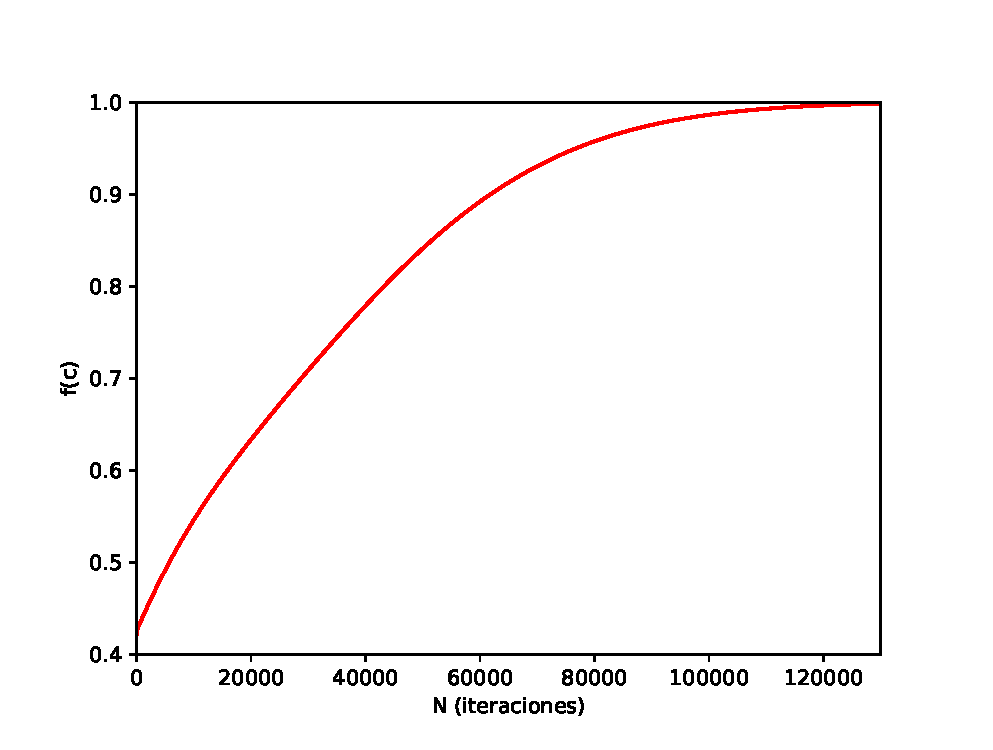
\includegraphics[width=0.40\textwidth]{figures/Graficas_Nuevas/Multi/FC.eps}
        }
    \subfigure[$f\left(x\right)=0.970$]{
        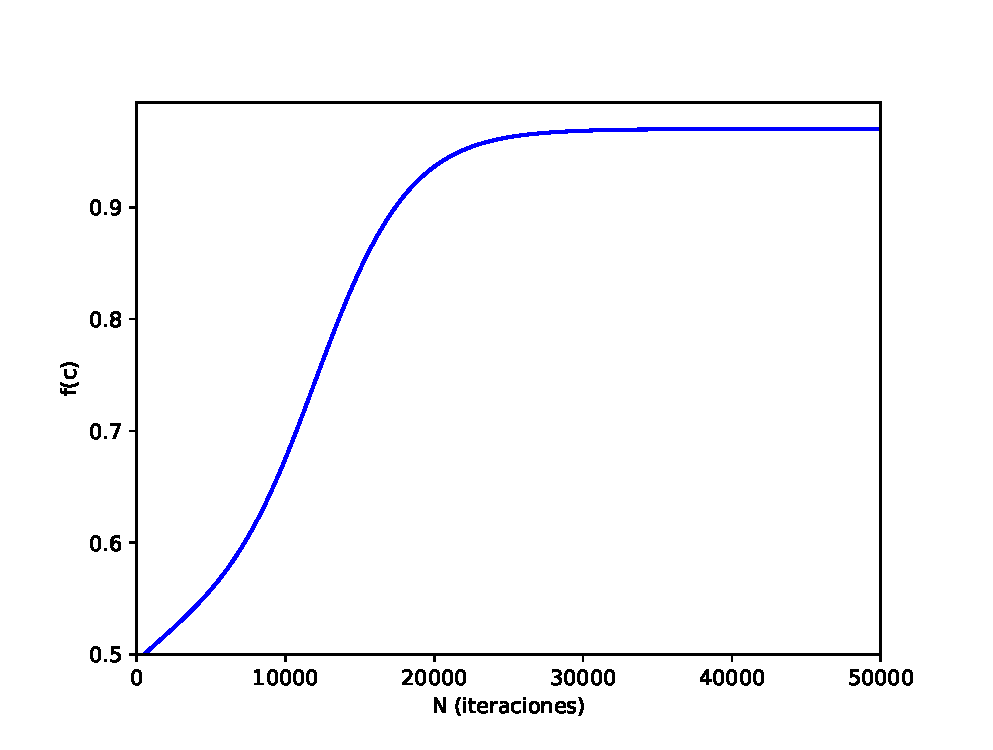
\includegraphics[width=0.40\textwidth]{figures/Graficas_Nuevas/Multi/f_99.eps}
        }
    \caption{Comparación del valor máximo de ambas fuentes}
    \label{Fun_Gauss_Multi}
  \end{center}
\end{figure}
Otro aspecto que se aprecia es el grosor de las componentes en la figura \ref{Comp_Multi_Gaussian}. Esto se puede asociar al error, traduciéndose en que si la estima del gradiente posee un error muy pronunciado el sistema tenderá a presentar oscilaciones.

\begin{figure}[H]
  \begin{center}
    \subfigure[Inicio en 0 0]{
        \includegraphics[width=0.40\textwidth]{figures/Graficas_Nuevas/Multi/00MULTI.eps}
        }
    \subfigure[Inicio en 0 800]{
        \includegraphics[width=0.40\textwidth]{figures/Graficas_Nuevas/Multi/Fun_3.eps}
        }
    \caption{Evaluación de las componentes del gradiente estimado según la fuente objetivo y el punto de partida}
    \label{Comp_Multi_Gaussian}
  \end{center}
\end{figure}






